\documentclass[landscape]{sintefposter}

\usepackage{hyperref,multicol,wrapfig}
\usepackage{tcolorbox}
\usepackage{fancyvrb}

\title{SpliPy$^{1.3}$ - Spline modelling in Python}

\author{Eivind Fonn, Kjetil Andre Johannessen }

\institute{SINTEF Digital, Dept. of Mathematics and Cybernetics, Trondheim, Norway}

\email{Eivind.Fonn@sintef.no, Kjetil.Johannessen@sintef.no}

\conference{SIN\TeX project}

\graphicspath{{.}{Figures/}}

\begin{document}
\leftlogo{splipylogo}
\maketitle

\begin{multicols}{3}
\section{Introduction}
\begin{tcolorbox}[colback=sintefblue!10!white,colframe=sintefblue,title=Abstract]
  Splipy is a pure python library for the creation, evaluation and manipulation of B-spline and NURBS geometries.
  It supports $n$-variate splines of any dimension, but emphasis is made on the use of curves, surfaces and volumes.
  The library is designed primarily for analysis use, and therefore allows fine-grained control over many aspects which is not possible to achieve with conventional CAD tools.
\end{tcolorbox}
\textbf{Keywords:} NURBS, B-splines, CAD, Interpolation, Approximation
\vspace{1cm}

\begin{tcolorbox}[colback=white,colframe=sintefblue,title=Installation]
  The package is distributed through the Python Package Index (PyPI) and can be installed by typing
  \begin{tcolorbox}[colback=sinteflightgrey]
  \begin{verbatim}
> pip install splipy \end{verbatim}
  \end{tcolorbox}
  into the commandline; or anaconda promt
\end{tcolorbox}

\vspace{-2cm}
\section{B-splines}
Given a knot vector of nondecreasing knots $\Xi=[\xi_1, \xi_2, \xi_3, ... \xi_{n+p+1}]$ we define the set of $n$ basisis functions by
\begin{tcolorbox}[colback=sintefblue!10!white,colframe=sintefblue,title=The basis]
  \begin{equation}
    \label{eq:bspline}
    N_{i,p}(\xi) = \frac{\xi - \xi_i}{\xi_{i+p}-\xi_i}N_{i,p-1}(\xi) + \frac{\xi_{i+p+1}-\xi}{\xi_{i+p+1}-\xi_{i+1}}N_{i+1,p-1}(\xi),
  \end{equation}
  and special casing the 0th order functions,
%  \begin{equation}
%    \label{eq:bspline-start}
%    N_{i,0}(\xi) = \left\{
%    \begin{array}{ll}
%      1  &  $if $ \ \ \xi \in [\xi_i, \xi_{i+1}) \\
%      0  &  $else$
%    \end{array}
%    \right.
%  \end{equation}
\end{tcolorbox}

By creating a tensor product of two or three univariate splines weighted by their controlpoints, we are able to create surface and solid representations.

\begin{center}
  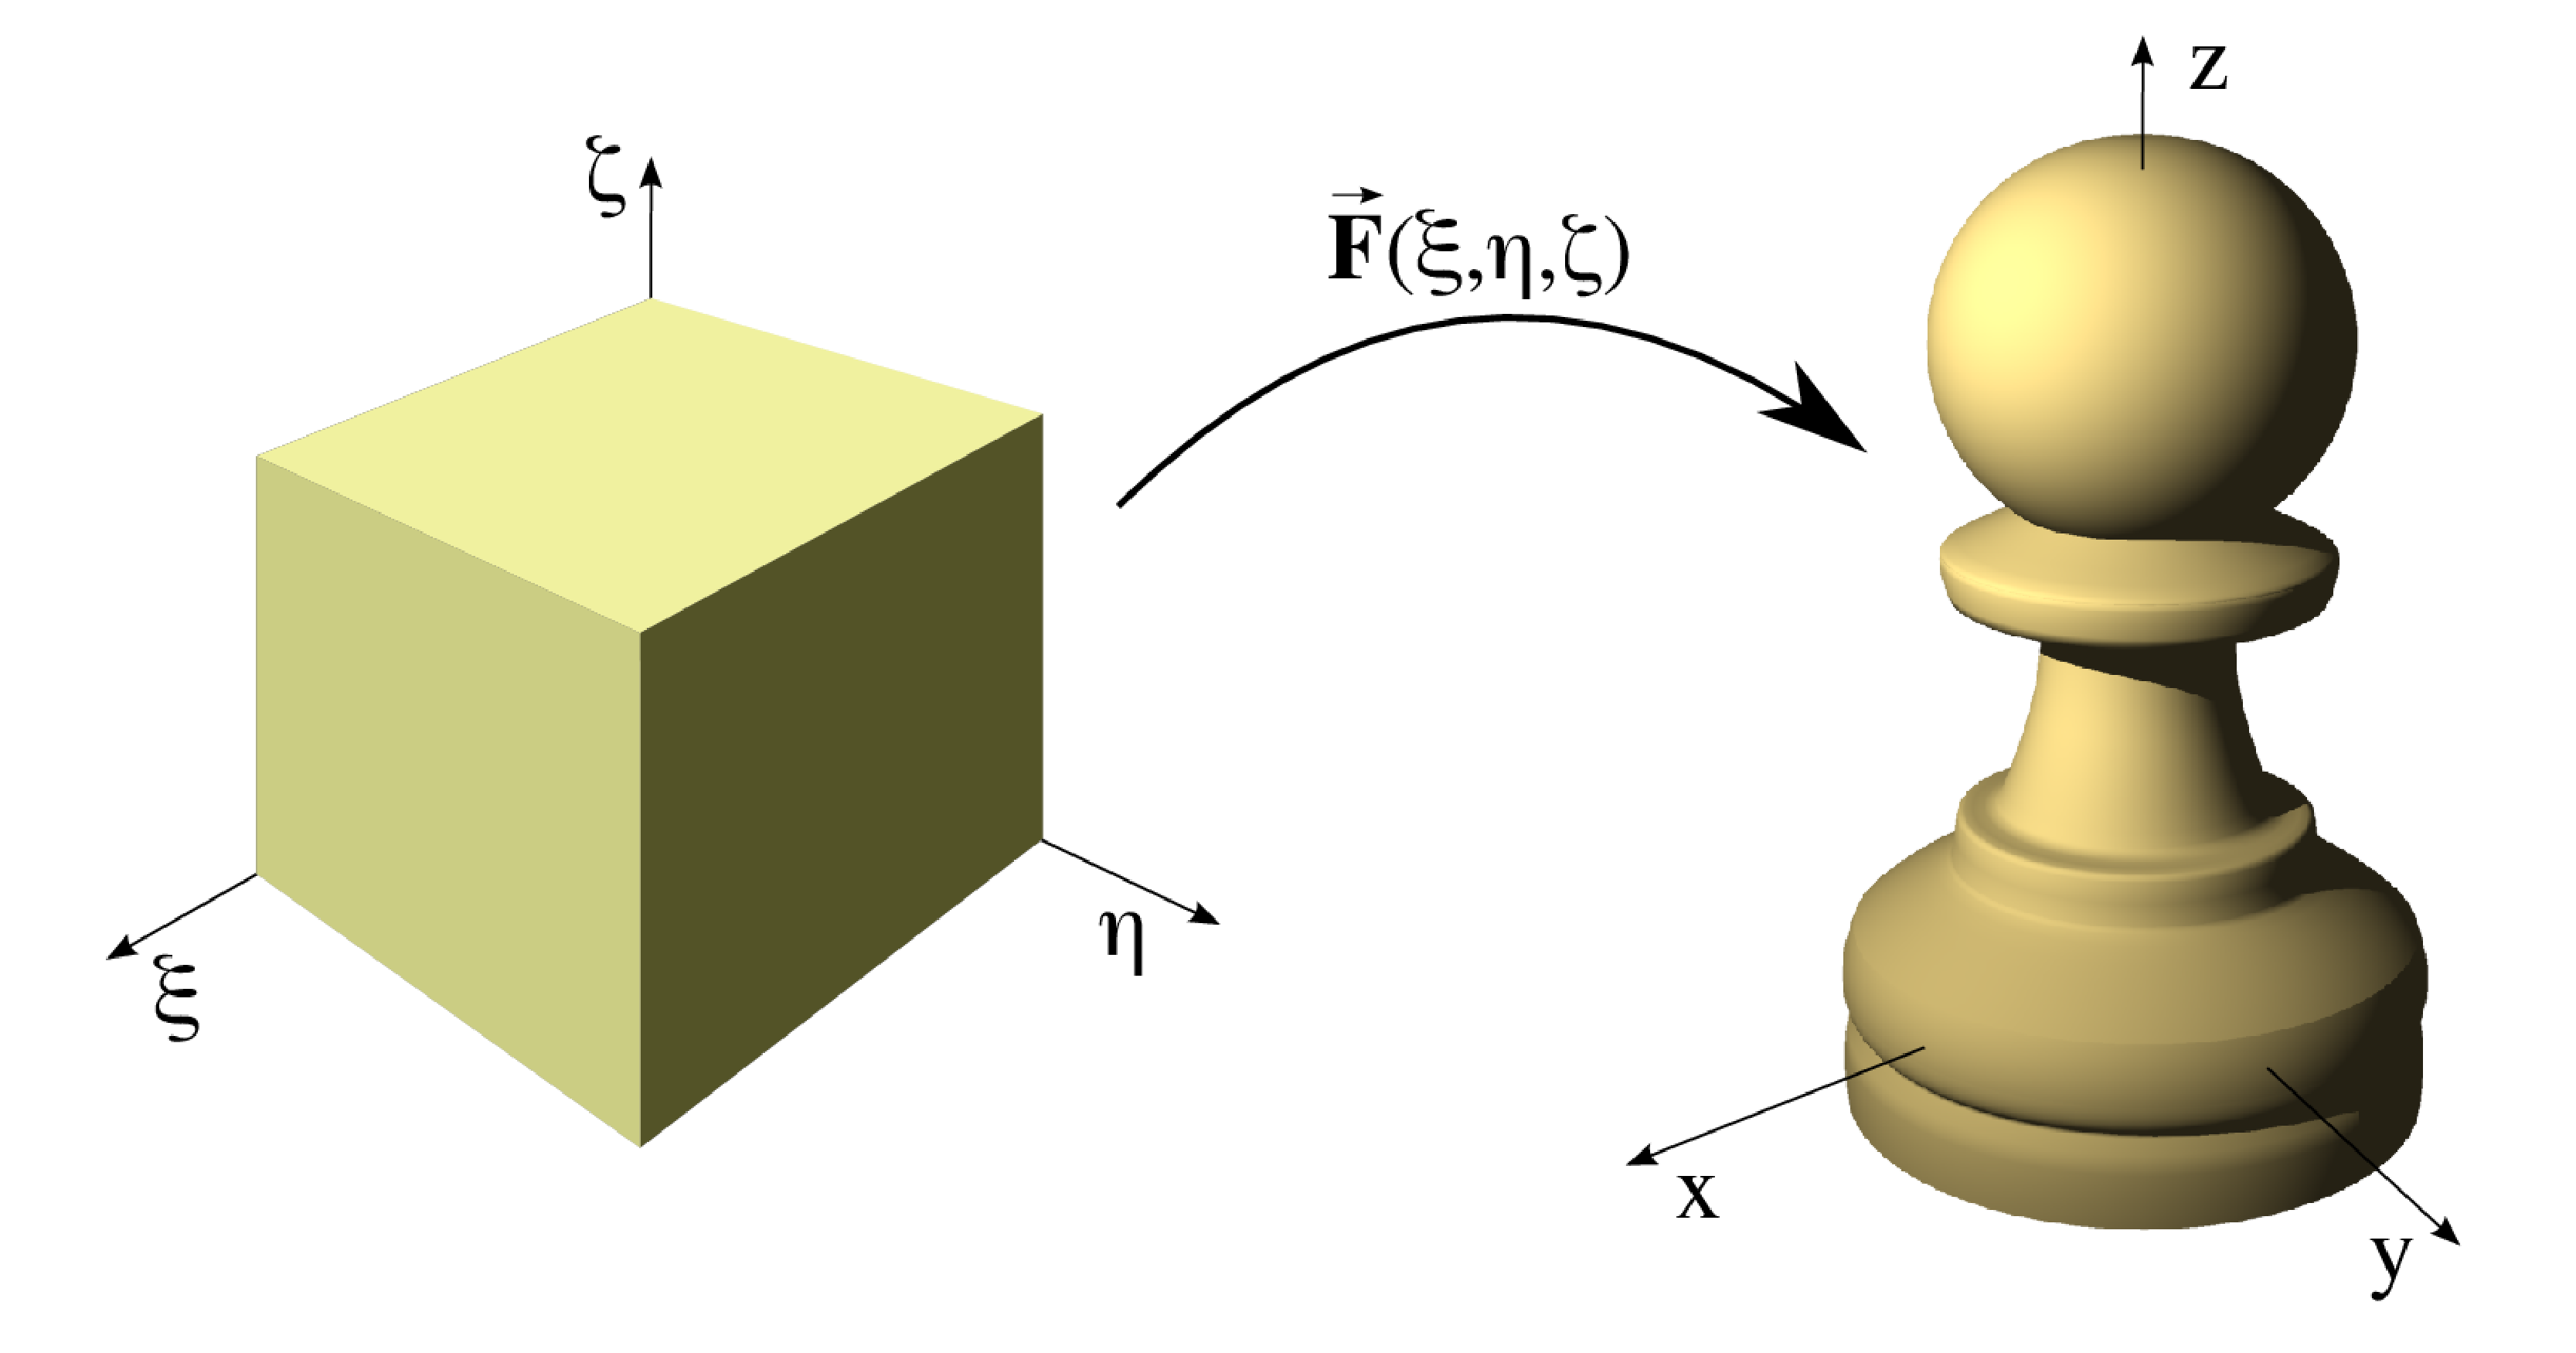
\includegraphics[width=16cm]{pawn-mapping}
  
\includegraphics[height=5cm]{MappingQR} \\
  \normalsize{Fig 1: A trivariate NURBS solid mapping}
\end{center}

\vspace{-1cm}
\section{Structure}

The class follows a simple structure with a Curve, Surface and Volume class which all inherit from a parent SplineObject class. Corresponding to each of these primtitives, we collect a number of generative methods in so-called factory classes.

\begin{center}
  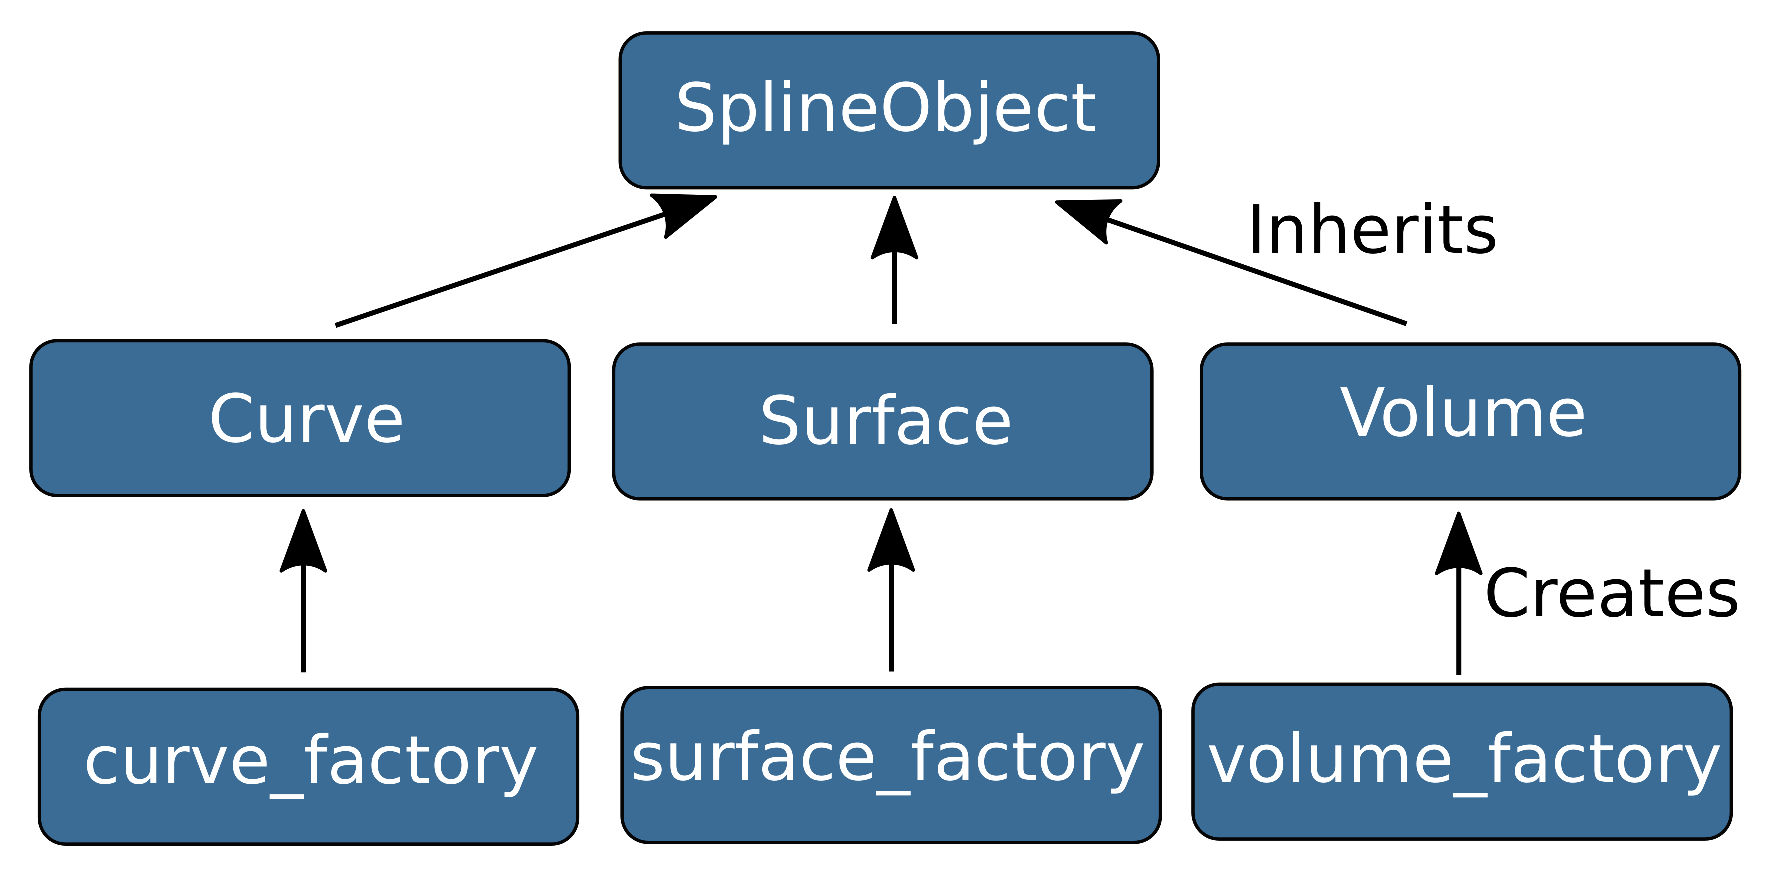
\includegraphics[width=0.7\linewidth]{classstructure} \\
  \normalsize{Fig 2: Primary classes and modules}
\end{center}

\vspace{-.5cm}
\section{Examples}

Adaptive curve fitting for parametric curves.
Uses a posteriori error estimate to refine where needed
\begin{tcolorbox}[colback=sinteflightgrey]
  \begin{Verbatim}[fontsize=\footnotesize]
from splipy import *
from numpy import pi,cos,sin,transpose,array

def trefoil(u):
  x = [    45*sin(u)- 30*cos(2*u)+113*sin(2*u)-11*cos(3*u)+27*sin(3*u),
 41*cos(u)-18*sin(u)- 83*cos(2*u)- 83*sin(2*u)-11*cos(3*u)+27*sin(3*u),
 36*cos(u)+27*sin(u)-113*cos(2*u)+ 30*sin(2*u)+11*cos(3*u)-27*sin(3*u)]
  return transpose(array(x))

knot_curve = curve_factory.fit(trefoil, 0, 2*pi)
  \end{Verbatim}
\end{tcolorbox}

\begin{figure}[ht]
  \begin{center}
    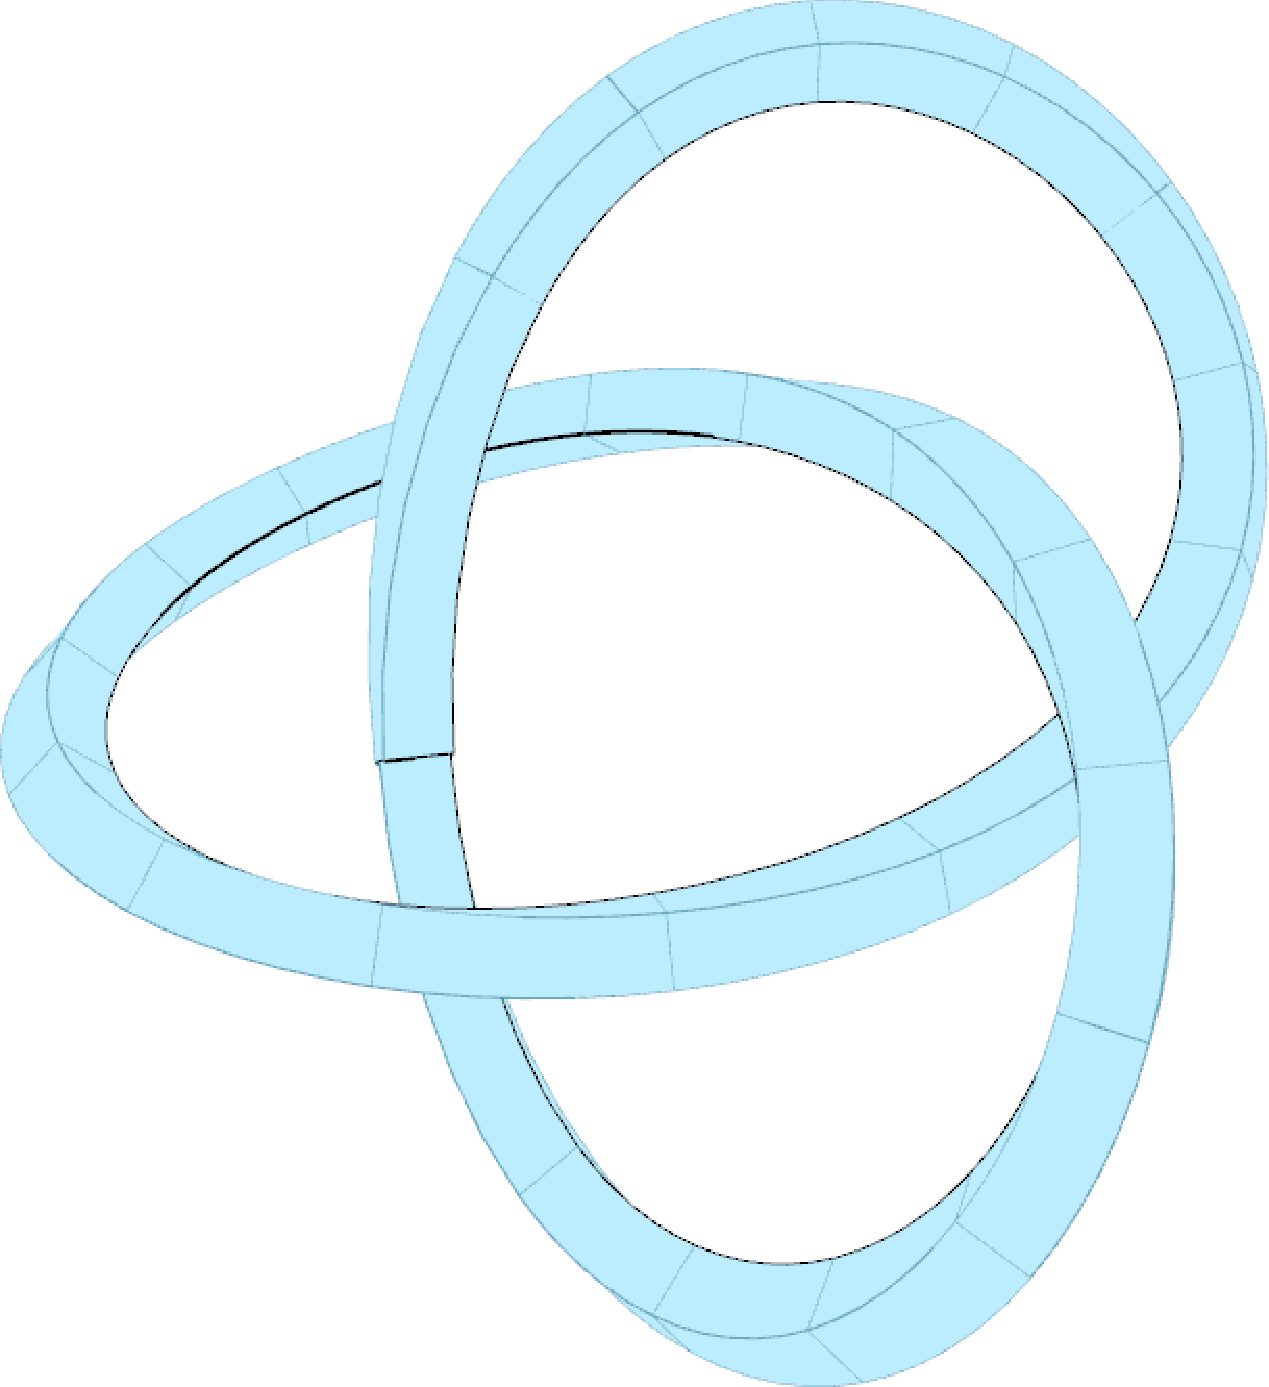
\includegraphics[width=0.24\textwidth]{trefoil}
  \end{center}
\end{figure}
Sweep operations where one curve is swept along another
\begin{tcolorbox}[colback=sinteflightgrey]
  \begin{Verbatim}[fontsize=\footnotesize]
square = 15*curve_factory.n_gon(4)
srf = surface_factory.sweep(knot_curve, square)
  \end{Verbatim}
\end{tcolorbox}




\begin{figure}[ht]
  \begin{center}
    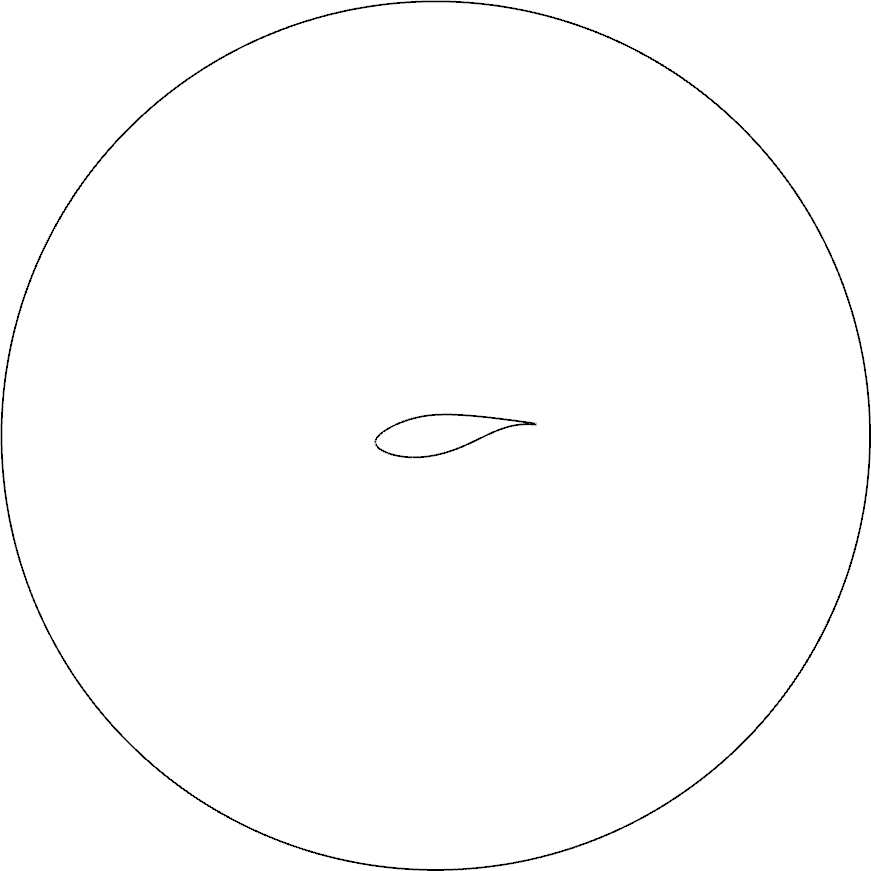
\includegraphics[width=0.24\textwidth]{Figures/tfi-1}
    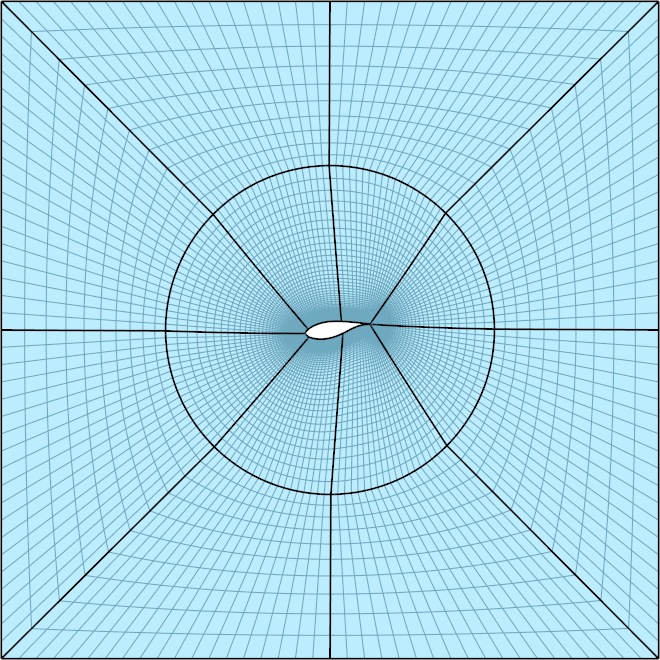
\includegraphics[width=0.24\textwidth]{Figures/tfi-4}
    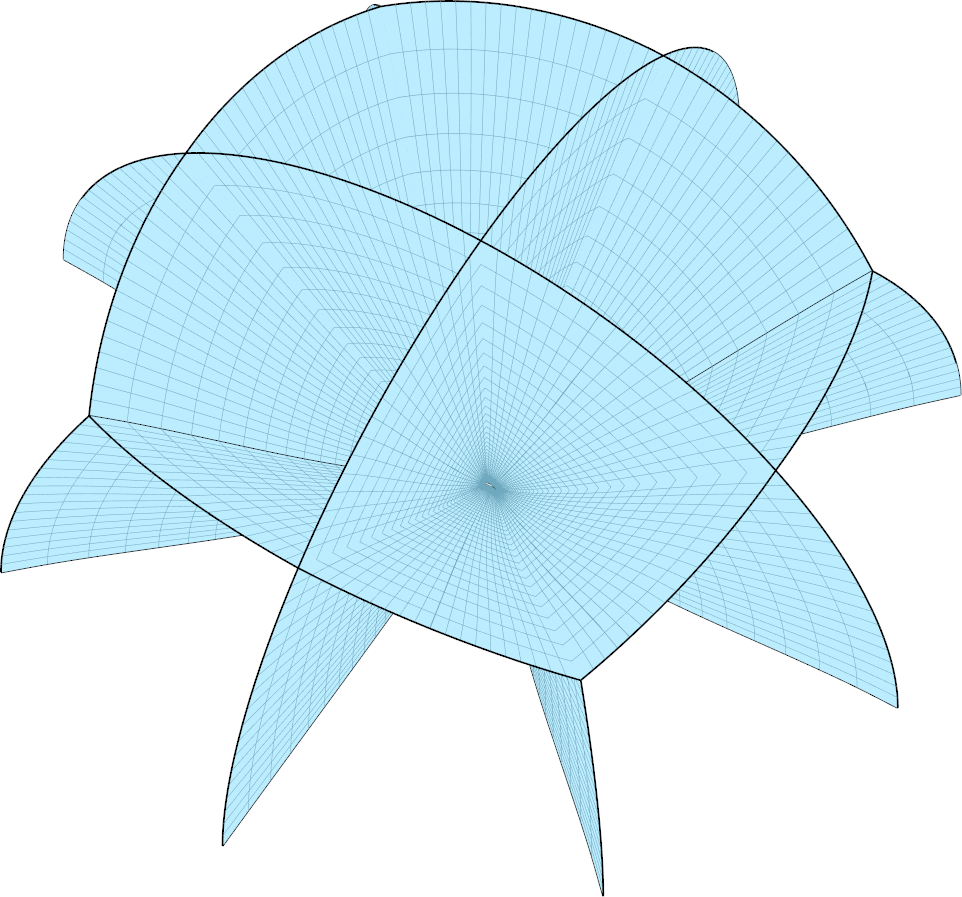
\includegraphics[width=0.24\textwidth]{Figures/wingtip-flower} \\
%    \small{
%      Fig 3: Line-to-surface construction of ``O-mesh'' around an airfoil.
%    }
%    \small{
%      Fig 4: Line-to-surface construction of a ``flower mesh'' around a wingtip.
%    }
  \end{center}
\end{figure}
\begin{figure}[ht]
  \begin{center}
    \raisebox{1.3cm}{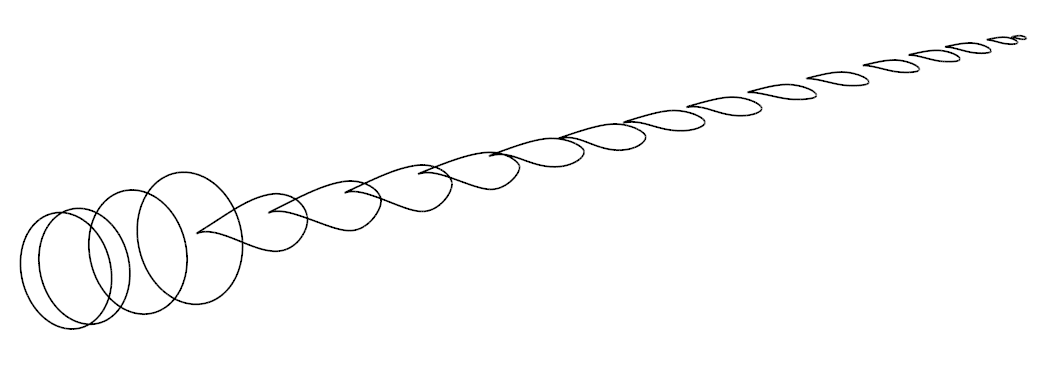
\includegraphics[width=0.32\textwidth]{Figures/cross-airfoils}}
    \raisebox{0.4cm}{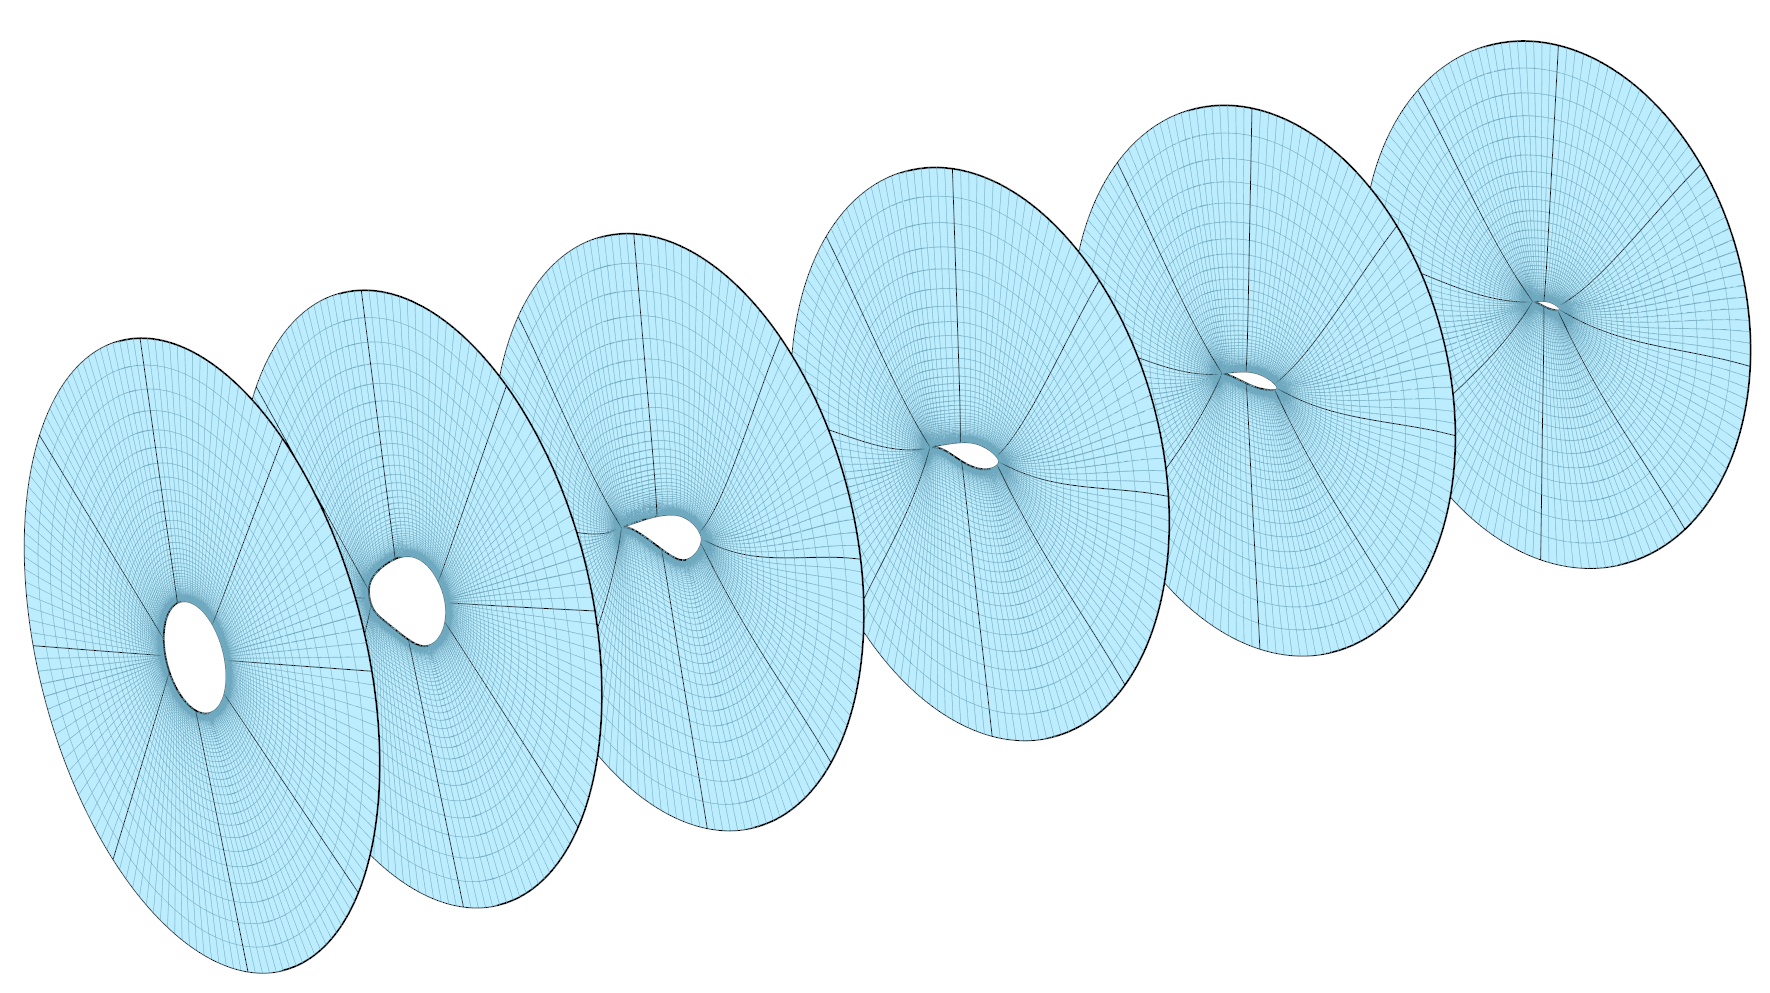
\includegraphics[width=0.32\textwidth]{Figures/crossecs2}}
    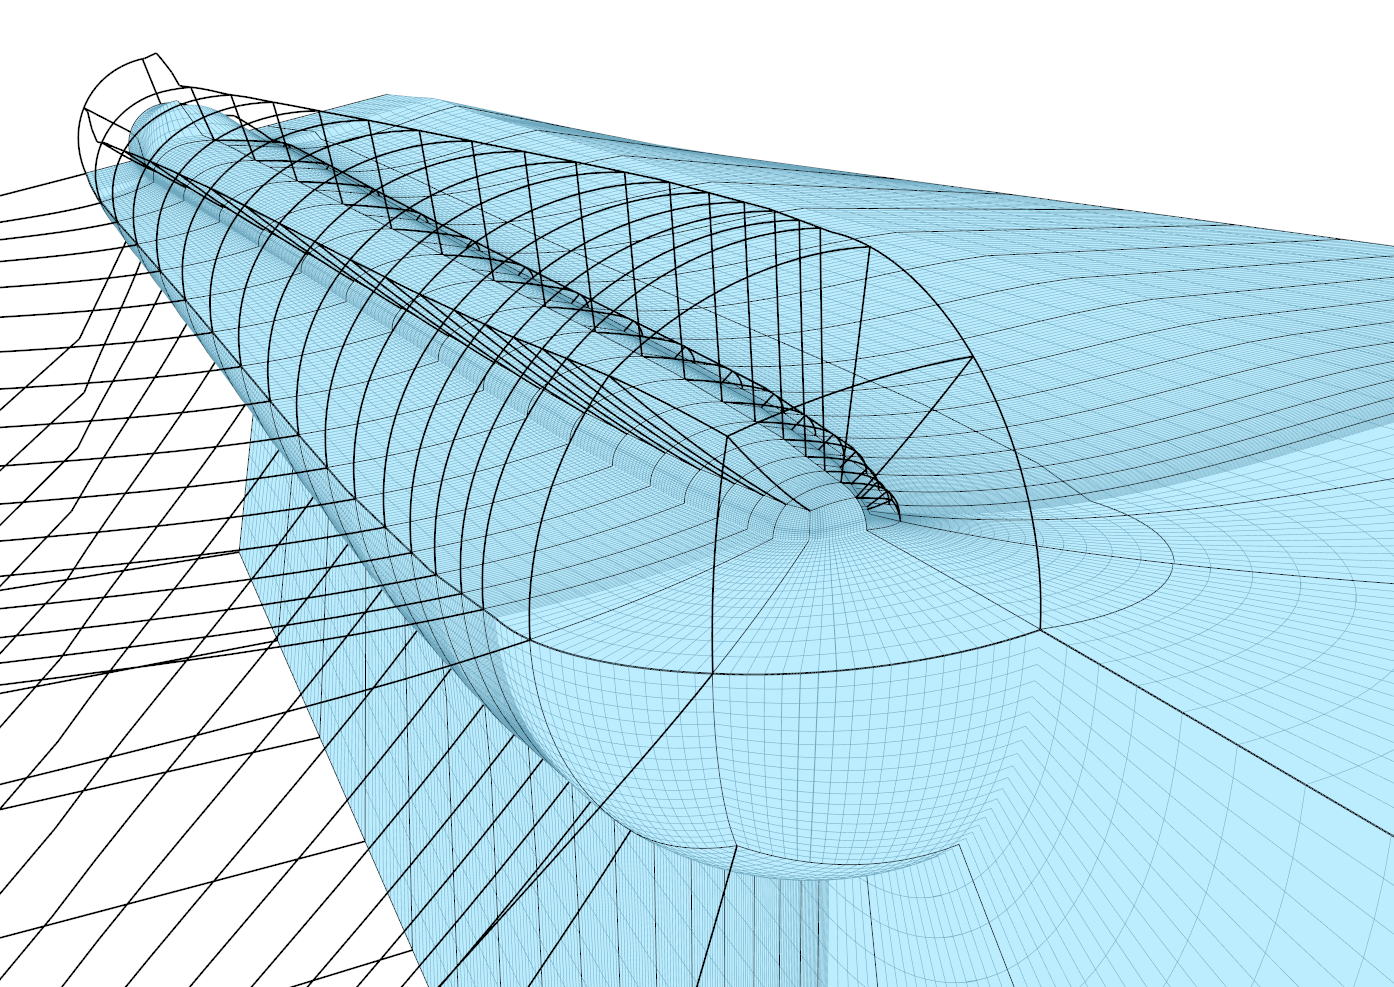
\includegraphics[width=0.32\textwidth]{Figures/block-2} \\
    \small{
      Fig 5: Line-to-volume construction of a full wind-turbine blade mesh.
    }
  \end{center}
\end{figure}

\begin{tcolorbox}[colback=white,colframe=sintefblue,title=Integration with Nutils]
  The package contains functions for converting to Nutils objects.
  \begin{tcolorbox}[colback=sinteflightgrey]
  \begin{Verbatim}[fontsize=\footnotesize]
from splipy import *
from nutils import *

surf = surface_factory.disc(r=2, type='square')
surf = surf.rebuild(p=3, n=20)
domain, geom = utils.nutils.splipy_to_nutils(surf)
ns = function.Namespace()
ns.x   = geom
ns.phi = domain.basis('spline', degree=2)
A = domain.integrate(ns.eval_ij('phi_i,k phi_j,k'), degree=3)
b = domain.integrate(ns.eval_i('phi_i sin(7 x_0)'), degree=3)
cons = domain.boundary.project(0, ns.phi, ns.x,     degree=3)
ns.w = A.solve(b, constrain=cons)
\end{Verbatim}
  \end{tcolorbox}
\end{tcolorbox}
\vspace{-1cm}
\begin{figure}
  \begin{center}
    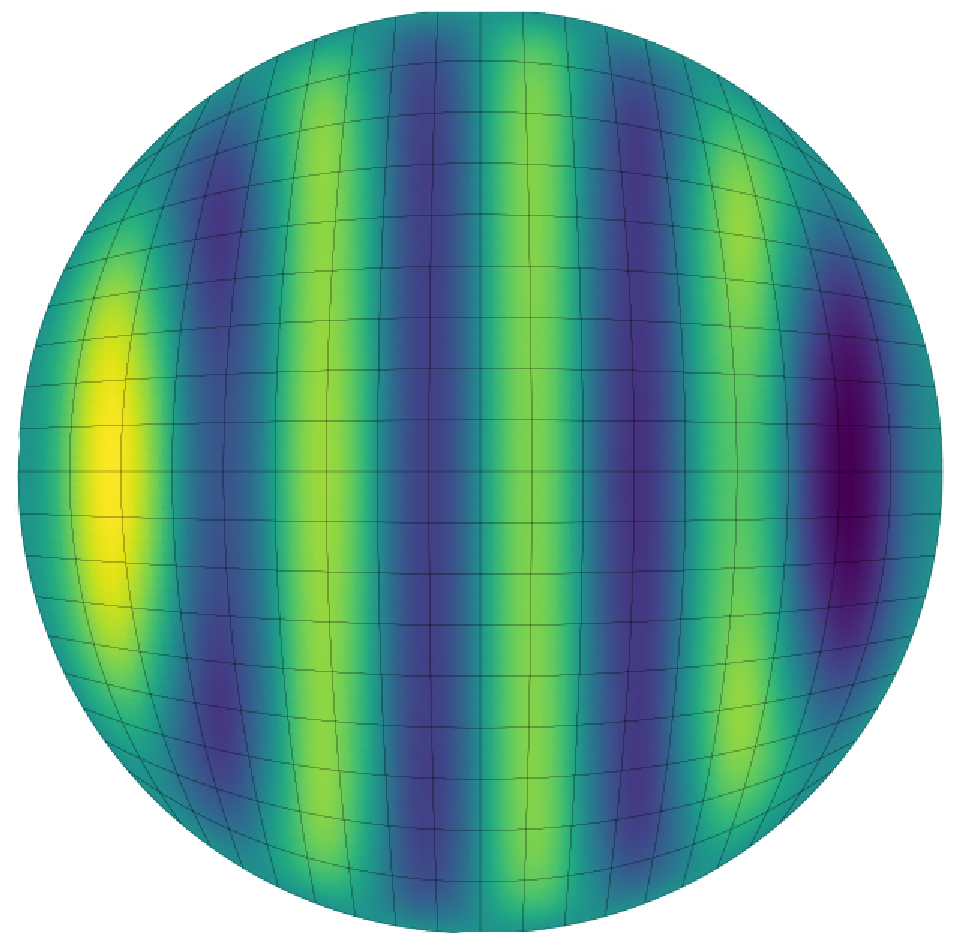
\includegraphics[width=0.24\textwidth]{nutilssolution}
    
\includegraphics[width=0.24\textwidth]{right.png} \\
    Solution $\quad\quad$ More nutils
  \end{center}
\end{figure}

\section{Conclusion}

Write som summary things here.
Maybe even box it all in.

{\footnotesize \textbf{Disclaimer:}
Splipy does not contain a graphical user interface.
All figures produced on this poster have been created using 3rd party visualizers.
Splipy is to be considered an API ready to be integrated into other custom applications.
}

\end{multicols}

\end{document}

